% !TEX root = ../arbeit.tex
\chapter{Evaluation}\label{chapter:evaluation}
To validate the fineness and quality of the proposed PROCAMS a technical evaluation was executed. In particular, the precision and speed of the pan-tilt unit were examined as well as the touch accuracy. Finally, overall performance of the PROCAMS is evaluated.
While planning the execution of larger usability studies in a domestic environment this evaluation should give a first clue of strengths and weaknesses of the build PROCAMS. 

\section{Pan-Tilt Unit Performance}
The task of the pan-tilt unit is to move the PROCAMS fast and accurate to a desired location. This two properties accuracy and pace were assessed in a laboratory study.

\subsection{Alignment Accuracy}
The accuracy approaching a previously stored position was determined by placing the PROCAMS with a distance of \SI{1}{\m} to a wall. The projector was displaying a red cross to indicate the centre of the projection. Then the pan-tilt unit was commanded to approach the stored position from eight defined starting points. The position where the red cross came to a standstill was marked at the wall.
Starting points were up, up-right, right, right-down, down, down-left, left, and left-up. Where up and down indicates a vertical shift by \SI{45}{\degree} from the stored position. Accordingly left and right indicates a horizontal shift by \SI{90}{\degree}. The measured distances in horizontal a vertical direction between the marked and stored position lead to an angel of aberration by simple trigonometry.
The stored position was approached ten times from each starting point. Thus 80 data points were obtained. A plot of the data is shown in~\autoref{plot:movement}.
% !TEX root = ../arbeit.tex
\begin{figure}[htbp]
        \centering
\tikzset{mark options={mark size=2, line width=1.5pt}}
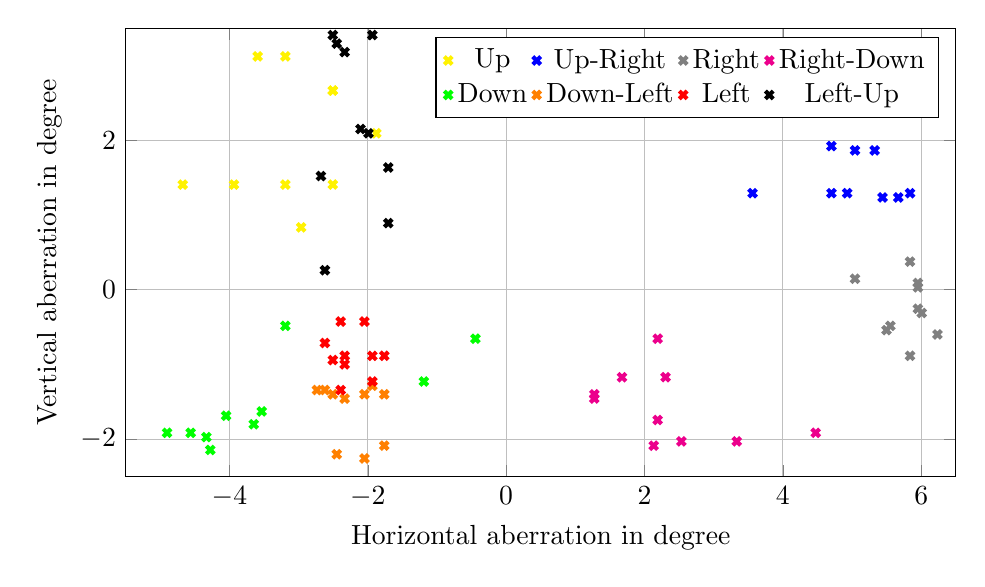
\begin{tikzpicture}
	\begin{axis}[%
	width=\textwidth,
	height = .6\textwidth,
	xmax = 6.5,
	xmin = -5.5,
	xstep= 1,
	ymin = -2.5,
	ymax =3.5,
	ystep=1,
	grid=major,
	legend columns=4,
	xlabel=Horizontal aberration in degree,
	ylabel=Vertical aberration in degree,
	scatter/classes={
		Up={mark=x,yellow},
		Up-Right={mark=x,blue},
		Right={mark=x,gray},
		Right-Down={mark=x,magenta},
		Down={mark=x,green},
		Down-Left={mark=x,orange},
		Left={mark=x,red},
		Left-Up={mark=x,black}
		}]
	\addplot[scatter,only marks,%
		scatter src=explicit symbolic]%
	table[meta=label] {
x     y      label
-4.67424872612533	1.40704466542326			Up
-3.93360909963853	1.40704466542326			Up
-3.1916505442666	1.40704466542326			Up
-2.9631282497019	0.834310816061917			Up
-2.50580769586769	1.40704466542326			Up
-1.87648177481699	2.09394419785448			Up
-2.50580769586769	2.66590922345048			Up
-3.59131574999252	3.12310419675389			Up
-3.1916505442666	3.12310419675389			Up
-2.50580769586769	2.66590922345048			Up
4.87197278490512	3.12310419675389			Up-Right
4.70128244616578	1.922268042484			Up-Right
5.04257648050957	1.8650348309974			Up-Right
5.32671540617036	1.8650348309974			Up-Right
5.44029823293142	1.23524883003786			Up-Right
5.66733440279074	1.23524883003786			Up-Right
5.83749482341844	1.29251672941418			Up-Right
4.70128244616578	1.29251672941418			Up-Right
4.92885045666407	1.29251672941418			Up-Right
3.56135251033059	1.29251672941418			Up-Right
5.83749482341844	-0.8844333423724			Right
5.49707362345356	-0.5407128664187			Right
5.55383818745301	-0.483421668036623			Right
6.23412919364215	-0.598002983536637			Right
5.950877911401	-0.254248352762198			Right
6.00755197509656	-0.311542730726946			Right
5.950877911401	0.0322288725769704			Right
5.950877911401	0.0895245826339467			Right
5.83749482341844	0.375998155486819			Right
5.04257648050957	0.146820113642666			Right
2.13256625938215	-2.08679175426757			Right-Down
3.33299828852148	-2.02956988177023			Right-Down
2.18978055419555	-1.74340203526284			Right-Down
1.27390493988743	-1.39988698938846			Right-Down
1.27390493988743	-1.45714715525241			Right-Down
1.67470826450442	-1.17081949820428			Right-Down
2.30419592354254	-1.17081949820428			Right-Down
2.18978055419555	-0.655291904866927			Right-Down
4.47356567736875	-1.9151140985677			Right-Down
2.53297060324095	-2.02956988177023			Right-Down
-4.90183476990765	-1.9151140985677			Down
-4.56039979299942	-1.9151140985677			Down
-4.33259451138178	-1.9723439586187			Down
-4.27562145717918	-2.14400946240445			Down
-3.64838313294688	-1.80064302302008			Down
-3.53424123132033	-1.62890972945458			Down
-3.1916505442666	-0.483421668036623			Down
-1.18943272767241	-1.22809016670015			Down
-0.444749555610536	-0.655291904866927			Down
-4.0476456276837	-1.68615756608216			Down
-2.44861895803739	-2.20122289252437			Down-Left
-2.04816744014753	-2.25843193102194			Down-Left
-1.76200574367305	-2.08679175426757			Down-Left
-2.7345115584368	-1.34262402653776			Down-Left
-2.62017007131273	-1.34262402653776			Down-Left
-2.50580769586769	-1.39988698938846			Down-Left
-2.33422694871262	-1.45714715525241			Down-Left
-2.04816744014753	-1.39988698938846			Down-Left
-1.76200574367305	-1.39988698938846			Down-Left
-1.93371422794441	-1.28535838089828			Down-Left
-2.62017007131273	-0.712579515900411			Left
-2.50580769586769	-0.941714567461968			Left
-2.33422694871262	-0.8844333423724			Left
-1.93371422794441	-0.8844333423724			Left
-1.76200574367305	-0.8844333423724			Left
-2.39142533786276	-1.34262402653776			Left
-1.93371422794441	-1.22809016670015			Left
-2.39142533786276	-0.426129502926883			Left
-2.04816744014753	-0.426129502926883			Left
-2.33422694871262	-0.998993909972118			Left
-2.62017007131273	0.261410180165005			Left-Up
-1.70476239345517	0.891593594551635			Left-Up
-2.67734348248654	1.5215613564293			Left-Up
-1.70476239345517	1.6360658892936			Left-Up
-1.99094282098346	2.09394419785448			Left-Up
-2.1053879716975	2.15116137745379			Left-Up
-2.33422694871262	3.1802267828006			Left-Up
-2.44861895803739	3.29445285887791			Left-Up
-2.50580769586769	3.40865272433571			Left-Up
-1.93371422794441	3.40865272433571			Left-Up
	};

\addlegendentry{Up}
\addlegendentry{Up-Right}
\addlegendentry{Right}
\addlegendentry{Right-Down}
\addlegendentry{Down}
\addlegendentry{Down-Left}
\addlegendentry{Left}
\addlegendentry{Left-Up}

	\end{axis}
\end{tikzpicture}
\caption{Aberration of the pan-tilt unit approaching a defined location}
\label{plot:movement}
\end{figure}

The average horizontal misalignment is \SI{3,29}{\degree}. For vertical alignment, the average error is \SI{1,48}{\degree}. Hence, the misalignment in an arbitrary direction is \SI{3,74}{\degree}. This accords to a shift of less than \SI{10}{\cm} if the \emph{surface} is \SI{150}{\cm} away from the projector.
A likely reason for the smaller misalignment in the vertical direction is caused by an additionally used accelerometer to control the servo for horizontal alignment. Since, for horizontal alignment no secondary sensor is used, the alignment is not as good. Overall the alignment is fair enough to re-project a widget at almost the same location in the physical world, but is not sufficient enough to augment small tangible objects as for example a light switch. 

A more accurate alignment could be achieved by two different modifications. On the one hand, a sensor providing very accurate data for horizontal and vertical alignment could be attached to provide feedback of the current alignment of the pan-tilt unit. Nonetheless, previous attempts already showed that a simple calibrated and compensated compass is not suitable for this task since the projector and servos have a strong influence on the magnetic field.

On the other hand, more powerful servos with a high resolution potentiometer could be installed. The potentiometer would lead the servo to move more precisely to the commanded position. This approach seems very promising without any major change at the pan-tilt unit. 

\subsection{Alignment Pace}
The pace of the pan-tilt unit was evaluated in a separate benchmark. Therefor, the time needed for \SI{164}{\degree} horizontal pan and a \SI{110}{\degree} tilt was measured. Each movement was repeated ten times from both directions. Since panning and tilting is performed simultaneously no combinations of tilt and pan were executed.

On average the pan-tilt unit needed \SI{3.5}{\second} for the horizontal pan task. For the tilt task, the unit needed \SI{4.8}{\second}. A reason for the slower tilt movement could be the higher force needed for tilting compared to the rotation force. Overall the PROCAMS can reach every position in less than \SI{6}{\second} (worst-case: move \SI{135}{\degree} vertically). This seems to be a decent time.
Of course, there are faster servos available, but higher acceleration forces could damage the printed case holding the PROCAMS. 


\section{Touch Performance}
Touch performance was evaluated in a basic laboratory study. The PROCAMS was mounted over a desk in a distance of \SI{75}{\cm}. It was tilted down \SI{70}{\degree} from horizontal, pointing at the desk illuminating an \textit{interaction space} of \SI{40 x 30}{\cm}. The setup is shown in~\autoref{img:evalSetup}. Four red crosses surround by a white circle posed as target. They were distributed on three different \textit{surfaces}. Two targets at the desk, one at the cardboard box on the left side and one on a ramp composed of a red notebook. The four targets are depicted in~\autoref{img:evalTargets}. In all cases, the diameter of the red cross was \SI{18}{\mm}.
\begin{figure}
        \centering
        \begin{subfigure}[b]{0.31\textwidth}
                \includegraphics[width=\textwidth]{images/evaluation/targets.png}
                \caption{Four target positions for touch evaluation}
                \label{img:evalTargets}
        \end{subfigure}
	\hfill         
        \begin{subfigure}[b]{0.31\textwidth}
                \includegraphics[width=\textwidth]{images/evaluation/setup.png}
                \caption{Evaluation setup: PROCAMS and touch targets }
                \label{img:evalSetup}
        \end{subfigure}
	\hfill          
        \begin{subfigure}[b]{0.31\textwidth}      
                \includegraphics[width=\textwidth]{images/evaluation/touch.png}
                \caption{Green border indicates a detected touch}
                \label{img:EvalTouchDetection}
        \end{subfigure}
        \caption{Touch accuracy evaluation setup}
        \label{fig:TouchEval}
\end{figure}

During the study participants had the task to touch the targets as accurately as possible. Participants were ordered to take as much time as needed. Forty targets were presented in a counterbalanced order, one at a time. A detected touch was indicated by a green border (see~\autoref{img:EvalTouchDetection}). After touching the target, it disappeared and appeared at one of the three other positions.
Time as well as touch position in projector and world coordinate system were monitored. From that data, the error in mm in the world coordinate system can be derived.  

Ten participants between 24 and 27 years took part in this study. Hence, 400 touch events were monitored. On average participants needed \SI{109}{\second} to touch all 40 target. In less than 1\% the touch was not detected on the first approach. This was counted manually. Distribution of monitored touch events for each target is shown in \autoref{fig:touchperformance}. The targets are labeled as follows: cardboard box (T1), ramp (T2), left desk(T3) and right desk (T4). 
% !TEX root = ../arbeit.tex
\begin{figure}[htbp]
        \centering
        \begin{subfigure}[b]{0.24\textwidth}
\begin{tikzpicture}
    \node[anchor=north west,inner sep=0] (image) at (-0.21,3.4) {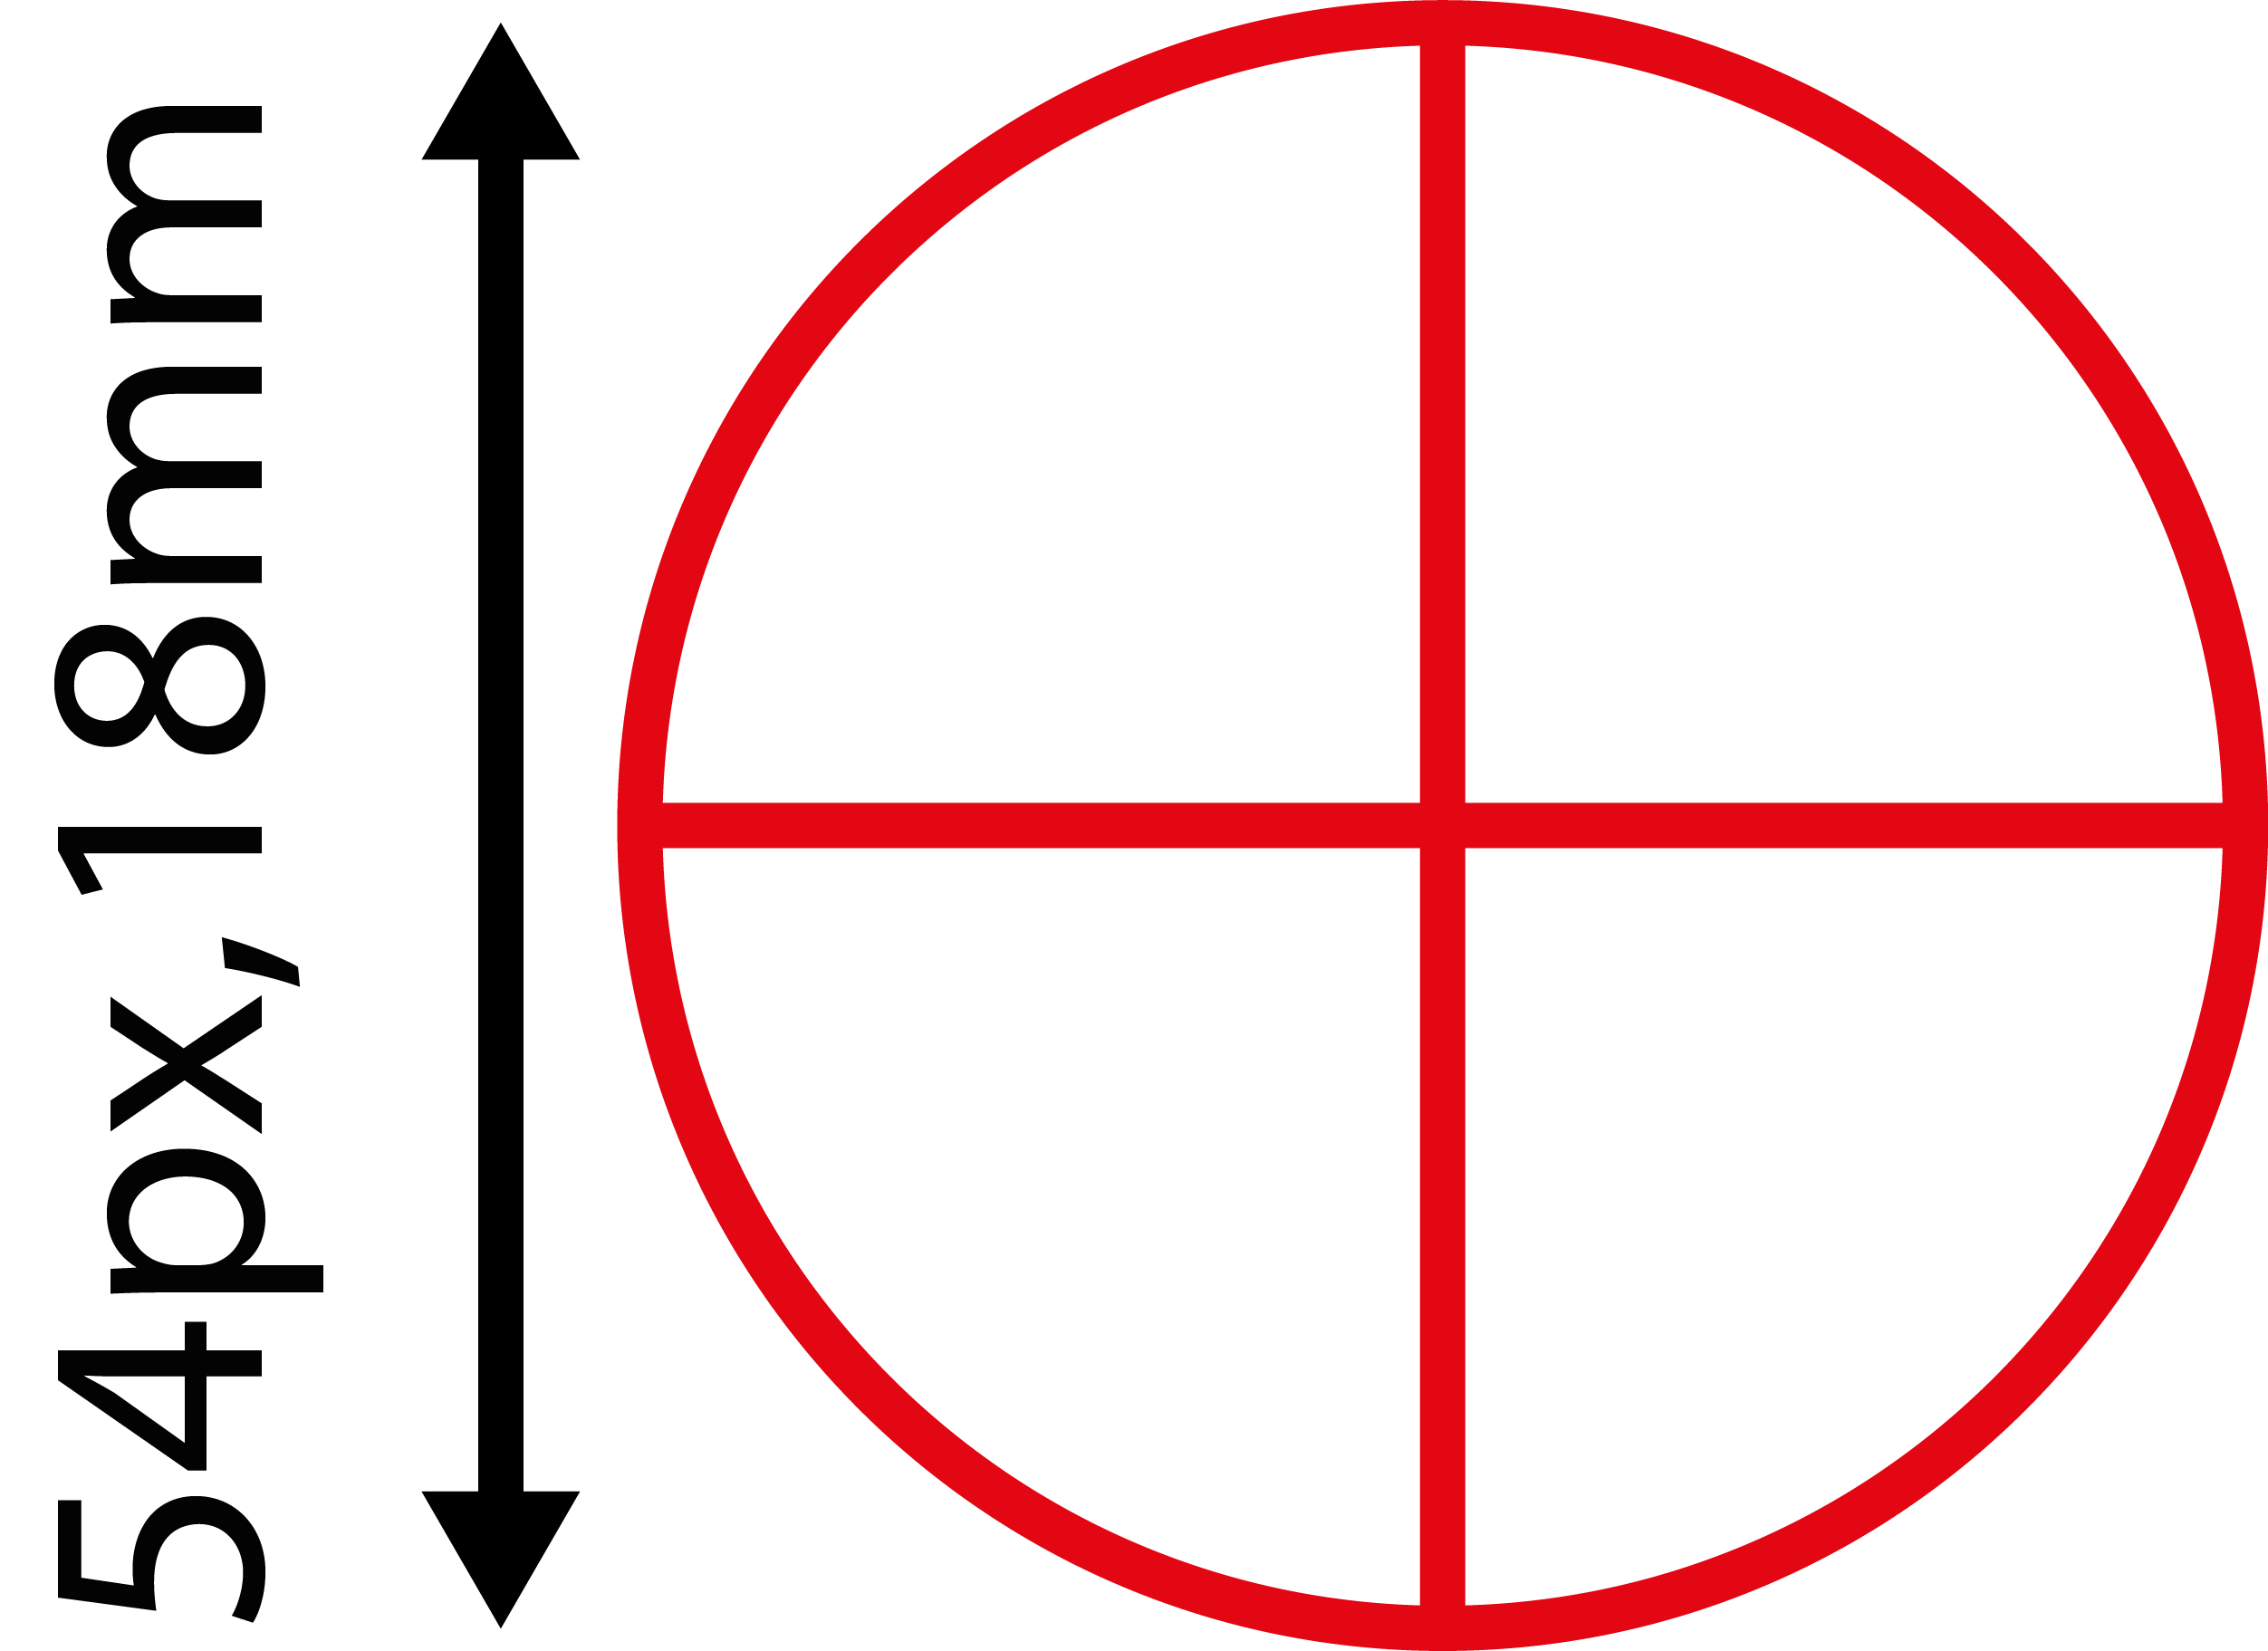
\includegraphics[width=.82\textwidth]{images/evaluation/target.png}};
    \begin{scope}[x={(image.south east)},y={(image.north west)}]
        	\begin{axis}[%
	width=1.2\textwidth,
	xmax = 25,
	xmin = -15,
	xstep= 1,
	ymin = -25,
	ymax =10,
	ystep=1,
	scale only axis,  hide axis,
	scatter/classes={
		touch={mark=x,blue},
		fix={mark=x,green}
		}]
	\addplot[scatter,only marks,%
		scatter src=explicit symbolic]%
	table[meta=label] {
x     y      label
11.4582	-13.3227333333333	touch
7.67326666666667	-7.4573	touch
13.7794666666667	-10.2132	touch
7.69923333333333	-10.1318666666667	touch
8.76113333333333	-14.6389666666667	touch
7.4581	-14.0683666666667	touch
11.1696333333333	-10.3373666666667	touch
12.4380333333333	-10.3844333333333	touch
10.7563333333333	-4.0675	touch
6.20993333333333	-11.5566333333333	touch
11.6883	-6.52456666666667	touch
10.5672333333333	-5.44256666666667	touch
10.7563333333333	-4.0675	touch
8.96886666666667	-7.81206666666667	touch
8.23516666666667	-3.971	touch
9.98656666666667	-10.9915666666667	touch
13.6086666666667	-10.0759	touch
9.62673333333333	-13.7913	touch
12.3409666666667	-10.0288333333333	touch
9.62673333333333	-13.7913	touch
11.8568333333333	-13.8725	touch
11.2054666666667	-8.93913333333333	touch
12.3409666666667	-10.0288333333333	touch
10.9394333333333	-11.0268	touch
11.0726	-9.9817	touch
14.4302	-11.1557666666667	touch
10.1167666666667	-7.50533333333333	touch
7.90096666666667	-7.422	touch
8.04816666666667	-8.75813333333333	touch
8.08476666666667	0.080635	touch
11.5224	-0.020401	touch
8.97713333333333	-2.40637333333333	touch
11.4720666666667	-11.3492333333333	touch
12.6588	1.34631333333333	touch
8.77163333333333	-3.8115	touch
8.81786666666667	-1.34581666666667	touch
8.81786666666667	-1.34581666666667	touch
8.81786666666667	-1.34581666666667	touch
8.77163333333333	-3.8115	touch
10.0697	-1.38218333333333	touch
5.2139	-2.29801333333333	touch
9.51433333333333	-7.37496666666667	touch
10.5683666666667	-8.8268	touch
9.51433333333333	-7.37496666666667	touch
10.7723666666667	-7.40966666666667	touch
15.2854333333333	-8.95526666666667	touch
9.66823333333333	-6.31423333333333	touch
9.87296666666667	-4.9031	touch
10.0561	-12.3857666666667	touch
9.40906666666667	-17.0136666666667	touch
10.8307333333333	-16.7234666666667	touch
13.3813	-15.7832666666667	touch
14.3105	-8.1803	touch
11.4890333333333	-10.8130666666667	touch
15.0264333333333	-12.0241333333333	touch
11.6178333333333	-8.04463333333333	touch
8.7778	-10.6825666666667	touch
10.3703	-9.36893333333333	touch
8.46253333333333	-14.5130666666667	touch
10.4431333333333	-6.94726666666667	touch
11.3136666666667	-11.8486333333333	touch
10.9030333333333	-14.273	touch
7.6572	-9.2353	touch
10.5464333333333	-8.3371	touch
13.3813	-15.7832666666667	touch
14.3105	-8.1803	touch
11.4890333333333	-10.8130666666667	touch
15.0264333333333	-12.0241333333333	touch
11.6178333333333	-8.04463333333333	touch
8.7778	-10.6825666666667	touch
10.3703	-9.36893333333333	touch
8.46253333333333	-14.5130666666667	touch
10.4431333333333	-6.94726666666667	touch
11.3136666666667	-11.8486333333333	touch
10.9030333333333	-14.273	touch
7.6572	-9.2353	touch
10.5464333333333	-8.3371	touch
14.7625333333333	-9.29363333333333	touch
13.298	-11.6487333333333	touch
6.5016	-14.0928666666667	touch
11.8258333333333	-14.0161333333333	touch
9.2085	-12.8309333333333	touch
11.7829	-4.2875	touch
11.6589	-12.9584666666667	touch
9.5361	-9.01146666666667	touch
10.6363	-2.84416666666667	touch
13.4788333333333	-10.6140666666667	touch
10.9325333333333	-9.08683333333333	touch
7.80556666666667	-12.7579333333333	touch
5.3456	-12.6299	touch
9.1848	-3.10585	touch
13.7194666666667	-9.2373	touch
11.3586	-6.68223333333333	touch
9.2085	-12.8309333333333	touch
5.3456	-12.6299	touch
10.6882666666667	-10.4653666666667	touch
8.9613	-14.2191333333333	touch
6.05786666666667	-12.7339333333333	touch
9.26416666666667	-8.74093333333333	touch
9.05163333333333	-10.2207666666667	touch
7.74503333333333	-10.1771333333333	touch
	};
	\end{axis}
    \end{scope}
\end{tikzpicture}
\vspace{-2em}
                \caption{Cardboard box}
                \label{plotcrap}
\end{subfigure}
          \hfill
        \begin{subfigure}[b]{0.24\textwidth}
\begin{tikzpicture}
    \node[anchor=north west,inner sep=0] (image) at (-0.21,3.4) {\includegraphics[width=.82\textwidth]{images/evaluation/targetonly.png}};
    \begin{scope}[x={(image.south east)},y={(image.north west)}]
        	\begin{axis}[%
	width=1.2\textwidth,
	xmax = 25,
	xmin = -15,
	xstep= 1,
	ymin = -25,
	ymax =10,
	ystep=1,
	scale only axis,  hide axis,
	scatter/classes={
		touch={mark=x,blue},
		fix={mark=x,green}
		}]
	\addplot[scatter,only marks,%
		scatter src=explicit symbolic]%
	table[meta=label] {
x     y      label
12.9295333333333	-15.0042333333333	touch
13.0833666666667	-11.6840333333333	touch
11.8062333333333	-11.6639333333333	touch
10.8449333333333	-14.1787	touch
14.3642666666667	-14.2317	touch
10.8490666666667	-10.5679333333333	touch
13.0826	-10.6037333333333	touch
14.3623	-13.1471333333333	touch
9.57476666666667	-9.10886666666667	touch
10.8478333333333	-11.6488666666667	touch
8.28126666666667	-14.1401	touch
10.5493666666667	-21.7204	touch
15.359	-22.9153333333333	touch
13.1118666666667	-21.8005	touch
14.0513666666667	-15.9332	touch
14.0513666666667	-15.9332	touch
17.5702	-17.0804666666667	touch
13.0934	-15.9034333333333	touch
15.3287	-15.9728666666667	touch
15.3121666666667	-12.1769	touch
15.3332333333333	-17.0109	touch
16.6062	-16.0125666666667	touch
14.0425	-13.5159	touch
15.2789333333333	-12.6055333333333	touch
17.0561	-17.2796666666667	touch
16.9697	-13.3713333333333	touch
10.7879666666667	-10.7355333333333	touch
14.2184333333333	-4.86073333333333	touch
14.3163666666667	-9.7717	touch
14.2393666666667	-5.90966666666667	touch
15.5822333333333	-8.7506	touch
14.3656	-12.2425333333333	touch
12.0603	-9.7115	touch
12.0793666666667	-10.7697	touch
16.5699333333333	-9.83186666666667	touch
15.5527	-7.34623333333333	touch
17.0797333333333	-18.3500333333333	touch
15.6786333333333	-13.338	touch
14.4150666666667	-14.7236666666667	touch
12.0412333333333	-8.65516666666667	touch
15.7608333333333	-17.2474333333333	touch
17.0797333333333	-18.3500333333333	touch
14.2376	-14.5668333333333	touch
14.3699333333333	-24.4363333333333	touch
10.7206333333333	-15.8828666666667	touch
9.43326666666667	-15.8511333333333	touch
10.7086333333333	-14.8293666666667	touch
11.9773666666667	-13.4591	touch
11.9773666666667	-13.4591	touch
14.2376	-14.5668333333333	touch
14.3699333333333	-24.4363333333333	touch
10.7206333333333	-15.8828666666667	touch
9.43326666666667	-15.8511333333333	touch
10.7086333333333	-14.8293666666667	touch
11.9773666666667	-13.4591	touch
11.9773666666667	-13.4591	touch
14.6576	-16.0484666666667	touch
15.6645	-17.5093666666667	touch
14.6769	-17.4776666666667	touch
11.9708	-11.3357333333333	touch
14.6287	-13.909	touch
13.2965	-12.4436	touch
15.6444	-16.0801	touch
13.2647666666667	-9.95823333333333	touch
13.2511666666667	-8.89516666666667	touch
14.6431333333333	-14.9780666666667	touch
13.2511666666667	-8.89516666666667	touch
11.9537333333333	-9.91646666666667	touch
14.6287	-13.909	touch
14.6431333333333	-14.9780666666667	touch
11.044	-16.2895	touch
13.2965	-12.4436	touch
14.6287	-13.909	touch
13.3283	-14.936	touch
15.6645	-17.5093666666667	touch
11.9537333333333	-9.91646666666667	touch
15.6071333333333	-15.0502	touch
7.48123333333333	-22.2602333333333	touch
12.1853	-17.4385333333333	touch
7.51196666666667	-14.9988	touch
8.4773	-8.12266666666667	touch
2.83031333333333	-10.4768666666667	touch
20.2422333333333	-11.6597666666667	touch
14.3743333333333	-11.6101333333333	touch
16.8420666666667	-17.4612	touch
11.2915333333333	-10.4765666666667	touch
11.3108666666667	-12.876	touch
21.9043333333333	-9.38586666666667	touch
10.3505333333333	-10.4524333333333	touch
12.5363	-9.48363333333333	touch
11.3026	-11.8465333333333	touch
13.7885666666667	-9.51606666666667	touch
11.2723	-8.0866	touch
13.7885666666667	-9.51606666666667	touch
	};
	\end{axis}
    \end{scope}
\end{tikzpicture}
\vspace{-2em}
                \caption{Ramp}
\end{subfigure}
                  \hfill
        \begin{subfigure}[b]{0.24\textwidth}
\begin{tikzpicture}
    \node[anchor=north west,inner sep=0] (image) at (-0.21,3.4) {\includegraphics[width=.82\textwidth]{images/evaluation/targetonly.png}};
    \begin{scope}[x={(image.south east)},y={(image.north west)}]
        	\begin{axis}[%
	width=1.2\textwidth,
	%height = \textwidth,
	xmax = 25,
	xmin = -15,
	xstep= 1,
	ymin = -25,
	ymax =10,
	ystep=1,
	scale only axis,  hide axis,
	scatter/classes={
		touch={mark=x,blue},
		fix={mark=x,green}
		}]
	\addplot[scatter,only marks,%
		scatter src=explicit symbolic]%
	table[meta=label] {
x     y      label
10.3679333333333	-17.1161666666667	touch
9.3127	-12.9594666666667	touch
12.6991333333333	-12.9763333333333	touch
10.4240333333333	-11.7381	touch
11.777	-11.7453666666667	touch
11.5320666666667	-10.5203666666667	touch
11.9335	-5.2524	touch
12.8825333333333	-10.5281666666667	touch
10.5184666666667	-10.5145333333333	touch
9.48443333333333	-6.4468	touch
15.6548	-4.87726666666667	touch
11.6250666666667	-9.29996666666667	touch
10.9259333333333	-15.3114333333333	touch
12.0491	-14.0701333333333	touch
9.8211	-12.4014333333333	touch
8.80493333333333	-12.3961333333333	touch
13.6448666666667	-11.1825666666667	touch
12.5389333333333	-8.29573333333333	touch
13.7480666666667	-9.9472	touch
13.5414	-12.4208666666667	touch
8.91413333333333	-11.1559666666667	touch
11.5667666666667	-10.6056666666667	touch
10.9569333333333	-9.75456666666667	touch
7.45573333333333	-6.59576666666667	touch
13.678	-8.09683333333333	touch
8.46853333333333	-9.67406666666667	touch
12.4252666666667	-6.75063333333333	touch
10.5128	-2.35234	touch
12.2538	-8.05173333333333	touch
8.29456666666667	-10.9771333333333	touch
12.0248333333333	-9.7891	touch
11.1867	-8.01793333333333	touch
15.9481333333333	-9.916	touch
13.8486666666667	-6.79496666666667	touch
14.3082666666667	-14.2426666666667	touch
14.8769666666667	-9.88136666666667	touch
13.9659	-16.8683666666667	touch
14.7471666666667	-8.1307	touch
16.1741333333333	-8.17586666666667	touch
14.5360333333333	-12.4959333333333	touch
14.7066	-11.1878	touch
8.6925	-5.3315	touch
12.4252666666667	-6.75063333333333	touch
5.80953333333333	-10.8955	touch
8.8848	-16.5168	touch
15.2996666666667	-9.66186666666667	touch
14.0338333333333	-8.4467	touch
14.6298	-17.7573333333333	touch
13.7007666666667	-16.5337333333333	touch
14.7307333333333	-16.5373666666667	touch
13.8362666666667	-14.9096666666667	touch
14.7307333333333	-16.5373666666667	touch
14.8651	-14.9138333333333	touch
12.7707666666667	-11.2612666666667	touch
15.0660333333333	-12.4852	touch
13.8362666666667	-14.9096666666667	touch
10.2671333333333	-12.4618333333333	touch
15.2996666666667	-9.66186666666667	touch
14.0338333333333	-8.4467	touch
14.6298	-17.7573333333333	touch
13.7007666666667	-16.5337333333333	touch
14.7307333333333	-16.5373666666667	touch
13.8362666666667	-14.9096666666667	touch
14.7307333333333	-16.5373666666667	touch
14.8651	-14.9138333333333	touch
12.7707666666667	-11.2612666666667	touch
15.0660333333333	-12.4852	touch
13.8362666666667	-14.9096666666667	touch
10.2671333333333	-12.4618333333333	touch
11.5870666666667	-7.50206666666667	touch
14.0411	-7.53213333333333	touch
13.8764666666667	-12.8591333333333	touch
8.6011	-12.7941333333333	touch
11.5870666666667	-7.50206666666667	touch
14.0411	-7.53213333333333	touch
11.7075333333333	-6.27866666666667	touch
16.6122	-6.33866666666667	touch
15.4435	-7.5493	touch
9.19046666666667	-3.397	touch
11.8679	-4.6503	touch
12.9893333333333	-7.51926666666667	touch
12.5898666666667	-11.6104666666667	touch
12.9893333333333	-7.51926666666667	touch
14.2046666666667	-2.23925666666667	touch
12.9893333333333	-7.51926666666667	touch
12.7584666666667	-6.29153333333333	touch
8.84706666666667	-10.3335333333333	touch
13.8764666666667	-12.8591333333333	touch
10.4139	-8.71436666666667	touch
13.9222333333333	-8.7574	touch
4.52396666666667	-17.6386	touch
7.23206666666667	-16.2353	touch
10.2079666666667	-10.0701333333333	touch
6.44683333333333	-11.443	touch
11.2597666666667	-12.9417666666667	touch
10.3759666666667	-11.4990333333333	touch
16.4497333333333	-11.5856333333333	touch
9.93356666666667	-14.8354	touch
16.2682	-13.0133666666667	touch
8.9471	-11.4786666666667	touch
9.1377	-10.0549333333333	touch
%9.93356666666667	-14.8354	touch
%11.4476666666667	-11.5143	touch
%13.0517666666667	-9.63156666666667	touch
%10.8476333333333	-7.0474	touch
%9.38906666666667	-9.55196666666667	touch
%11.8465666666667	-7.06913333333333	touch
%11.9442666666667	-11.7814	touch
%11.7741666666667	-8.51683333333333	touch
%12.9974666666667	-10.7173333333333	touch
%9.38906666666667	-9.55196666666667	touch
%14.3836333333333	-9.66053333333333	touch
%9.5592	-12.8165333333333	touch
%11.7198666666667	-9.6026	touch
%14.1230666666667	-8.20556666666667	touch
	};
	\end{axis}
    \end{scope}
\end{tikzpicture}
\vspace{-2em}
                \caption{Left desk}
\end{subfigure}
                  \hfill
        \begin{subfigure}[b]{0.24\textwidth}
\begin{tikzpicture}
    \node[anchor=north west,inner sep=0] (image) at (-0.21,3.4) {\includegraphics[width=.82\textwidth]{images/evaluation/targetonly.png}};
    \begin{scope}[x={(image.south east)},y={(image.north west)}]
        	\begin{axis}[%
	width=1.2\textwidth,
	%height = \textwidth,
	xmax = 25,
	xmin = -15,
	xstep= 1,
	ymin = -25,
	ymax =10,
	ystep=1,
	scale only axis,  hide axis,
	scatter/classes={
		touch={mark=x,blue},
		fix={mark=x,green}
		}]
	\addplot[scatter,only marks,%
		scatter src=explicit symbolic]%
	table[meta=label] {
x     y      label
14.1284666666667	-14.0482333333333	touch
17.6497	-12.7129666666667	touch
13.8801666666667	-8.41066666666667	touch
13.357	-17.3332	touch
9.83086666666667	-12.2969666666667	touch
12.0485666666667	-13.4364666666667	touch
12.034	-12.2639333333333	touch
13.2899333333333	-12.2450666666667	touch
13.2745	-11.0751666666667	touch
13.2745	-11.0751666666667	touch
12.0194333333333	-11.093	touch
11.1045666666667	-13.4514	touch
14.2840666666667	-16.1396666666667	touch
12.0194333333333	-11.093	touch
11.1232	-15.0183	touch
8.1875	-11.9042666666667	touch
15.127	-14.4117333333333	touch
16.4382	-14.4176333333333	touch
12.8847333333333	-17.2995	touch
15.0665666666667	-11.5300333333333	touch
14.1428333333333	-14.4073	touch
14.1179333333333	-13.1701333333333	touch
14.1179333333333	-13.1701333333333	touch
14.1428333333333	-14.4073	touch
13.7101	-13.2174666666667	touch
10.8004666666667	1.63396666666667	touch
15.0436666666667	-11.8681	touch
12.2791666666667	-11.8304666666667	touch
9.7188	-7.2682	touch
13.6613666666667	-11.8493	touch
13.7101	-13.2174666666667	touch
12.3257333333333	-13.1985666666667	touch
16.0281666666667	-10.5181333333333	touch
13.8736666666667	-17.809	touch
16.133	-13.2505666666667	touch
17.6458666666667	-16.4791	touch
15.2139333333333	-16.4456333333333	touch
16.6036666666667	-13.2047	touch
14.2892	-14.4320333333333	touch
16.6317333333333	-14.4426333333333	touch
14.2636	-13.1932	touch
9.19043333333333	-10.2836333333333	touch
12.9248666666667	-13.1866	touch
11.6076	-14.4199333333333	touch
12.9489666666667	-14.4259666666667	touch
16.6036666666667	-13.2047	touch
14.2892	-14.4320333333333	touch
16.6317333333333	-14.4426333333333	touch
14.2636	-13.1932	touch
9.19043333333333	-10.2836333333333	touch
12.9248666666667	-13.1866	touch
11.6076	-14.4199333333333	touch
12.9489666666667	-14.4259666666667	touch
12.3826	-13.7262333333333	touch
13.7091666666667	-13.7324333333333	touch
13.6847666666667	-12.5098333333333	touch
14.6441	-10.8892333333333	touch
13.6847666666667	-12.5098333333333	touch
14.6779333333333	-12.5148666666667	touch
16.9003666666667	-8.47406666666667	touch
9.96963333333333	-8.42993333333333	touch
12.2529333333333	-6.82926666666667	touch
10.9616	-8.43623333333333	touch
13.5475333333333	-5.6303	touch
13.6038333333333	-8.4531	touch
12.2529333333333	-6.82926666666667	touch
13.6038333333333	-8.4531	touch
12.3061	-9.6592	touch
13.6280666666667	-9.66713333333333	touch
12.3061	-9.6592	touch
12.2302	-5.62073333333333	touch
10.0378333333333	-12.4913333333333	touch
14.7033666666667	-13.7371	touch
12.3596	-12.5031333333333	touch
15.9387666666667	-9.68093333333333	touch
12.3596	-12.5031333333333	touch
12.4287	-16.1803	touch
14.6441	-10.8892333333333	touch
14.4600666666667	-11.0224333333333	touch
10.9388	-18.3827666666667	touch
14.4782	-12.3186	touch
8.5497	-10.9888	touch
10.8665666666667	-12.2997333333333	touch
7.26243333333333	-14.0166666666667	touch
10.8511666666667	-11.0019	touch
13.1889	-14.0439333333333	touch
13.1889	-14.0439333333333	touch
8.56336666666667	-12.2877333333333	touch
12.1646	-11.0093666666667	touch
12.6428666666667	-13.7407	touch
13.5781666666667	-9.96786666666667	touch
12.5959666666667	-9.95673333333333	touch
11.2732333333333	-8.8099	touch
13.5781666666667	-9.96786666666667	touch
9.9399	-6.53546666666667	touch
12.6147	-11.4684	touch
9.9399	-6.53546666666667	touch
12.5819333333333	-8.8247	touch
8.9831	-8.78403333333333	touch
	};
	\end{axis}
    \end{scope}
\end{tikzpicture}
\vspace{-2em}
                \caption{Right desk}
\end{subfigure}
\caption{Touch accuracy evaluation}
\label{fig:touchperformance}
\end{figure}




Collected touch data was analysed with a standard weighted-means ANOVA test (F=57.06, p<0.0001)  in conjunction with a  Tukey's honest significance test.
The mean touch error, variance and standard deviation for the different targets is specified in~\autoref{tab:touchErrorEval}.

In this study setup, T1 has a significantly smaller error than T2, T3 and T4 (p<0.01, HSD[.01]=1.3). This coincides with \textcite{Hardy:2012jo} results, who identify that the accuracy of touch detection mainly depends on sensor distance. Target 1 was closest to the camera. The significantly worse result of T2 in comparison to T3 and T4 (p<0.01, HSD[.01]=1.3) cannot be explained by distance since it was very similar. A likely reason could be the material and colour of the notebook, but further investigations are necessary. 

\begin{table}[htb]
\begin{tabularx}{\textwidth}{ l|XXXl}
\toprule
Target & T1 & T2 & T3 & T4 \\
\midrule
Mean (in mm) & 14.1104 & 19.3232 & 16.5835 & 17.82 \\
Variance & 8.4757 & 12.4966 & 8.5013 & 7.5729 \\
Std. deviation (in mm) & 2.9113 & 3.5351 & 2.9157 & 2.7519 \\
Significant versus & T2,T3,T4 & T3,T4 \\
\bottomrule
\end{tabularx}
\caption{Statistical data}
\label{tab:touchErrorEval}
\end{table}

A mean error of less than \SI{20}{\mm} requires large buttons for pleasant interaction. However, the small standard deviation for all targets is remarkable. It appears that for the evaluation setup a fixed offset between executed and detected touch was present. It is necessary to figure out how and where this offset emerged and if the offset could be correct. 
The offset could accrue at several positions in the processing pipeline. First of all a bad calibration file between the projector and camera could lead to errors. Although, this is unlikely since a new calibration file was created before the evaluation. A likely reason for non optimal detection could be the different field of views of projector and depth sensing camera. The projected image fills only an area of approximately \SI{340x220}{px} which is roughly $\sfrac{1}{4}$ of the available resolution. To improve this issue a projector with a short throw lens or a camera with zoom lens should be used to adapt the field of views. Finally, a non-conform transformation matrix could result in the error. A source code recheck could clarify this concern.

\subsection{Touch Pace}
Even though the depth sensing camera runs at 30 \ac{fps} on average only 21.8 fps are processed. In particular, processing limitations and the Qt event-queue are responsible for that loss of frames. Due to the used tracking users must press a target for at least three frames which is equivalent to \SI{0.138}{\second}. In the study it was only problematic for the first one or two targets since participants know instant detection from their smart phones. After explaining to interact slightly slower participants could interact in an enjoyable way. 


\section{Overall Performance}
Overall, the proposed PROCAMS performs well. Widgets are rendered with up to 30 fps.
As mentioned before, touch detection runs at almost 22 fps. This performance remains also when two to three individual widgets are added to different \textit{surfaces}. Adding more widgets will decrease the available processing power and touch detection slows down to 10 to 14 fps. This forces the user to interact in an unnatural slow way. For more synchronous rendered content alternative rendering techniques or more processing power are required. 

\section{Conclusion}
To assess the quality and performance of the build PROCAMS an evaluation was conducted. Pan-tilt unit and touch detection were analysed in separate studies. The pan-tilt unit fulfils the requirements and can approach a stored position in a short space of time. However, accuracy of the servos could be more accurate. Numerous possibilities of improvement were discussed.

Touch detection accuracy is very reasonable with a small standard deviation of less than \SI{3.5}{\mm}. Touch accuracy is comparable to other PROCAMS requiring a manual calibration task. Enabling touch detection on arbitrary surfaces without any setup specific calibration was a tough task. Mapping of detected touch points back to the projection makes is even more prone to failure. From this point of view and considering inexpensive hardware the touch accuracy is very auspicious.